So for this problem, we can represent the matrix $n\times n$ as a bipartite graph where we have $n$ nodes on one side, representing the rows and $n$ other nodes on the other side, representing the column. A "1" represent an edge linking its column and row.\\
For a bipartite graph $G = (\{U, V\}, E)$, nodes in $U$ representing the columns and nodes in $V$ representing the rows. Let's denote a node $U_i$ the one representing the $i$-th column and $V_i$ the one representing the $i$-th row.\\
\begin{figure}[here]
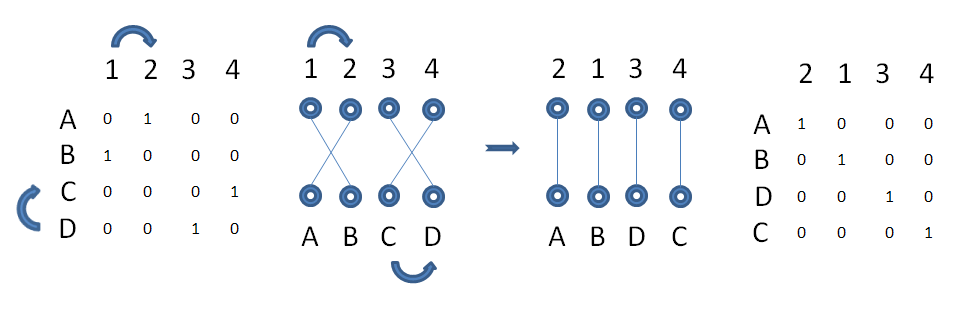
\includegraphics[scale=0.5]{matrix-matching}
\caption{Illustration of swapping colums and rows}
\label{fig:matrix-matching}
\end{figure}
As we can see on Figure~\ref{fig:matrix-matching}, to have a diagonalized matrix we need to have an edge linking $U_i$ and $V_i$, $\forall i \in \{1,2,\dots,n\}$. Plus swapping column $i$ with column $j$ means that $U_i$ becomes $U_j$ and $U_j$ becomes $U_i$. Same logic can be apply to swap rows. So if we have $n$ matching, it means we can diagonalize the matrix by swapping the columns and rows so we end up with $n$ edges linking $U_i$ with $V_i$, $\forall i \in \{1,2,\dots,n\}$. Thus our algorithm would just check if the matrix has $n$ matchings.